\documentclass{article}

\usepackage{a4wide}
\usepackage{graphicx}
\usepackage{subfig}
\usepackage{url}

\newcommand{\GOAL}{\textsc{Goal} }


%
%
%
\begin{document}

\title{The Wumpus World}
\author{Koen V. Hindriks and Wouter Pasman}
\maketitle

%
%
%
\section{Introduction}
%
The Wumpus World is a well-known two-dimensional grid that is
distributed with the \GOAL agent programming language and consists of cells
occupied by walls, pits, and green ground areas, see Figure
\ref{fig:wumpusStart}. The Wumpus World is called so because there is one
special grid cell that is occupied by the Wumpus, an ugly and dangerous beast.
There is also a single agent located somewhere on the grid looking for the pile
of gold that is present on one of the cells of the grid.
The Wumpus World is a variation of the more classical well-known grid
worlds such as the Tileworld \cite{Pol90}.

The aim of this document is to introduce the Wumpus World, the actions that
the agent can perform and the percepts that it will receive from the Wumpus World environment. For
comparison and more information about the Wumpus World, you can also have a look
at the discussion of this environment in \cite{Rus03}.

\begin{figure}[h]
\centering
\subfloat[Wumpus World loaded at start]{
	\label{fig:wumpusStart}
	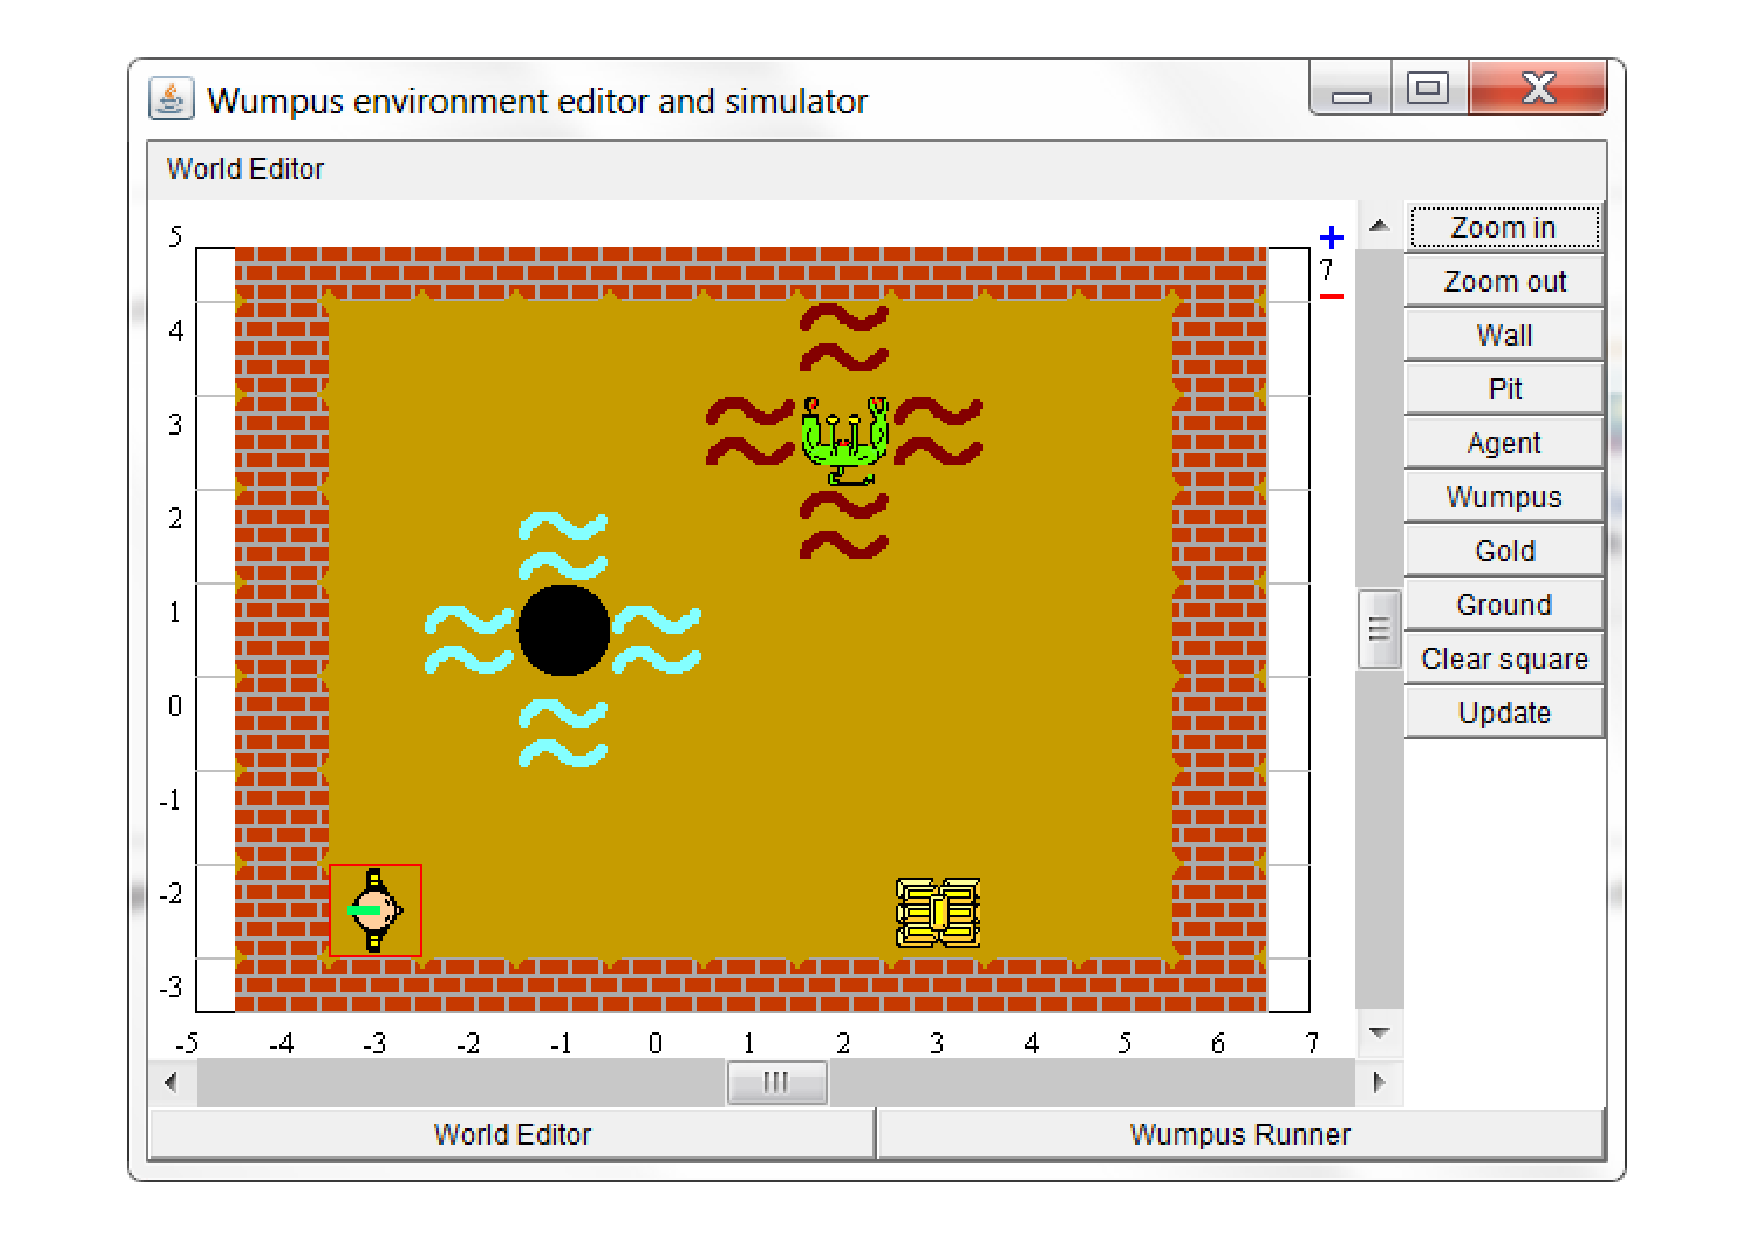
\includegraphics[width=7.5cm]{Figures/wumpusStart.pdf}
}
\subfloat[Initial Wumpus World grid]{
	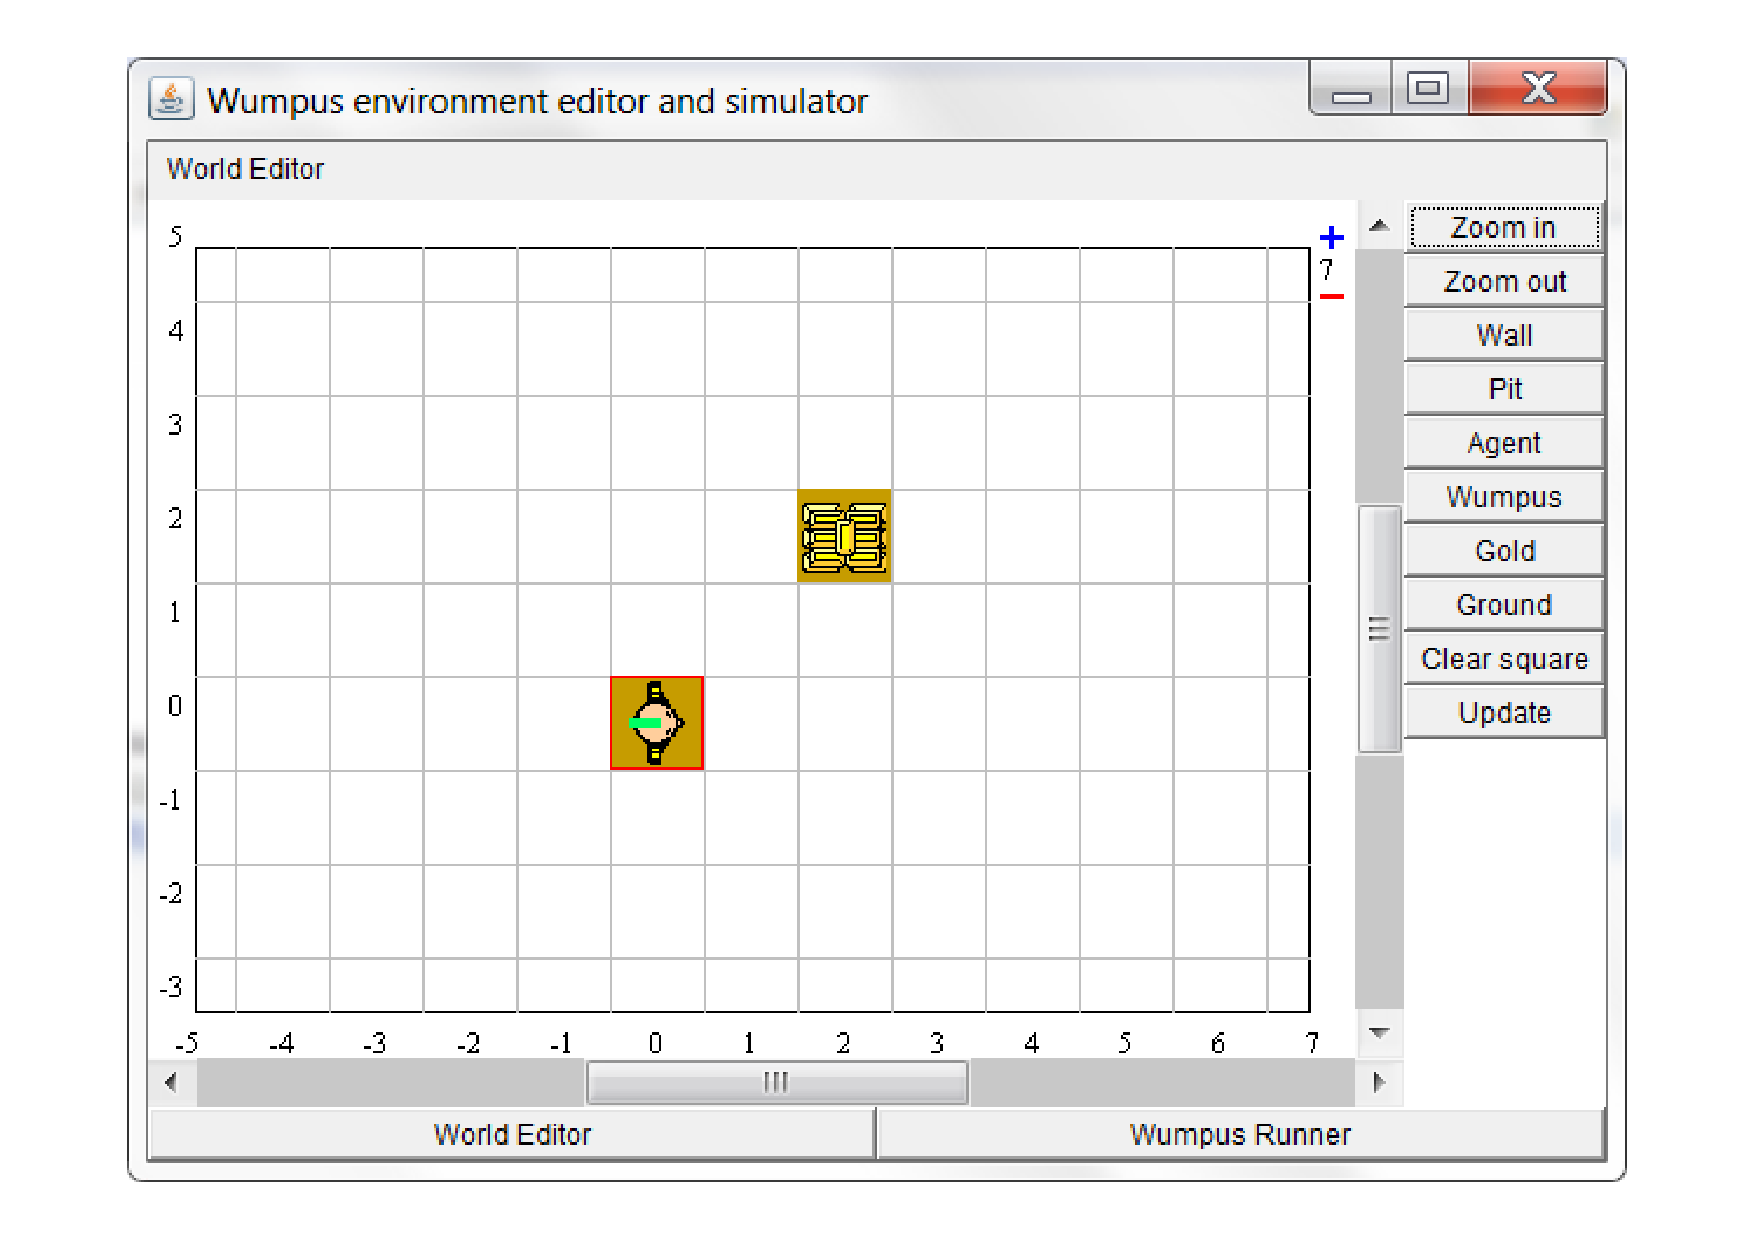
\includegraphics[width=7.5cm]{Figures/wumpusStartEmpty.pdf}
	\label{fig:wumpusStartEmpty}
}
\end{figure}


%
%
%
\section{Creating and Modifying Wumpus Worlds}
%
Right after you have launched the Wumpus World, a window appears that shows a
Wumpus World grid. When the Wumpus World environment is lauched a
Wumpus World may be loaded immediately from file, as shown in Figure
\ref{fig:wumpusStart}. If no World is loaded initially, the World Editor starts with a more or less
empty grid with only the agent and the pile of gold on it, as shown in Figure
\ref{fig:wumpusStartEmpty}.

This window is called the \textit{World Editor}, as is also indicated by the
label at the top left of the window. In the World Editor you can modify, load,
and save worlds. By clicking on the \textit{World Editor} item at the top left a
two-item menu appears that allows you to load or save a world. If you want to load
a world file, you need to locate \verb|.wld| files using a file browser.
Figure \ref{fig:wumpusStart} shows the \verb|wumpus.wld| file. Select the save
option in the menu to save any grid that you created.

You can modify and create your own worlds by selecting an item you want to
put on the grid with the buttons on the right hand side in the World Editor. You
can select either a wall, a pit, the agent, the Wumpus, a pile of gold,
or ground. After selecting an item, you can click on a grid cell to put the
item on that cell. You can also drag and select an entire area on the
grid in order to fill it with ground or walls.\footnote{Note that a breeze is shown
graphically on the grid but is only visible against a green background; the
breeze itself is white and does not show on an empty white cell.} By selecting
the \textit{Clear square} button, you can clear either individual cells or selected areas.


The editor ensures that at most one agent, one Wumpus, and one pile
of gold are present in any world. It does not ensure however that each of these
items is present. It thus is possible to create grids that do not satisfy the
basic requirements of a Wumpus World. Worlds that lack either an agent, a
Wumpus, or a pile of gold are said to be \textit{invalid}.


%
%
%
\section{Running the Agent in the Wumpus World}
%
From the World Editor you can switch to run mode by clicking the button
labeled \textit{Wumpus Runner}, see Figure \ref{fig:wumpusRunner}. The
environment will not accept actions if it is in edit mode. However, when running
the Wumpus World environment from \GOAL this switch is automatic when a
multi-agent system is started and there is no need to press the button. Of
course, for getting back to the World Editor the \textit{World Editor} button at
the bottom left needs to be pressed again.

\begin{figure}[h]
\centering
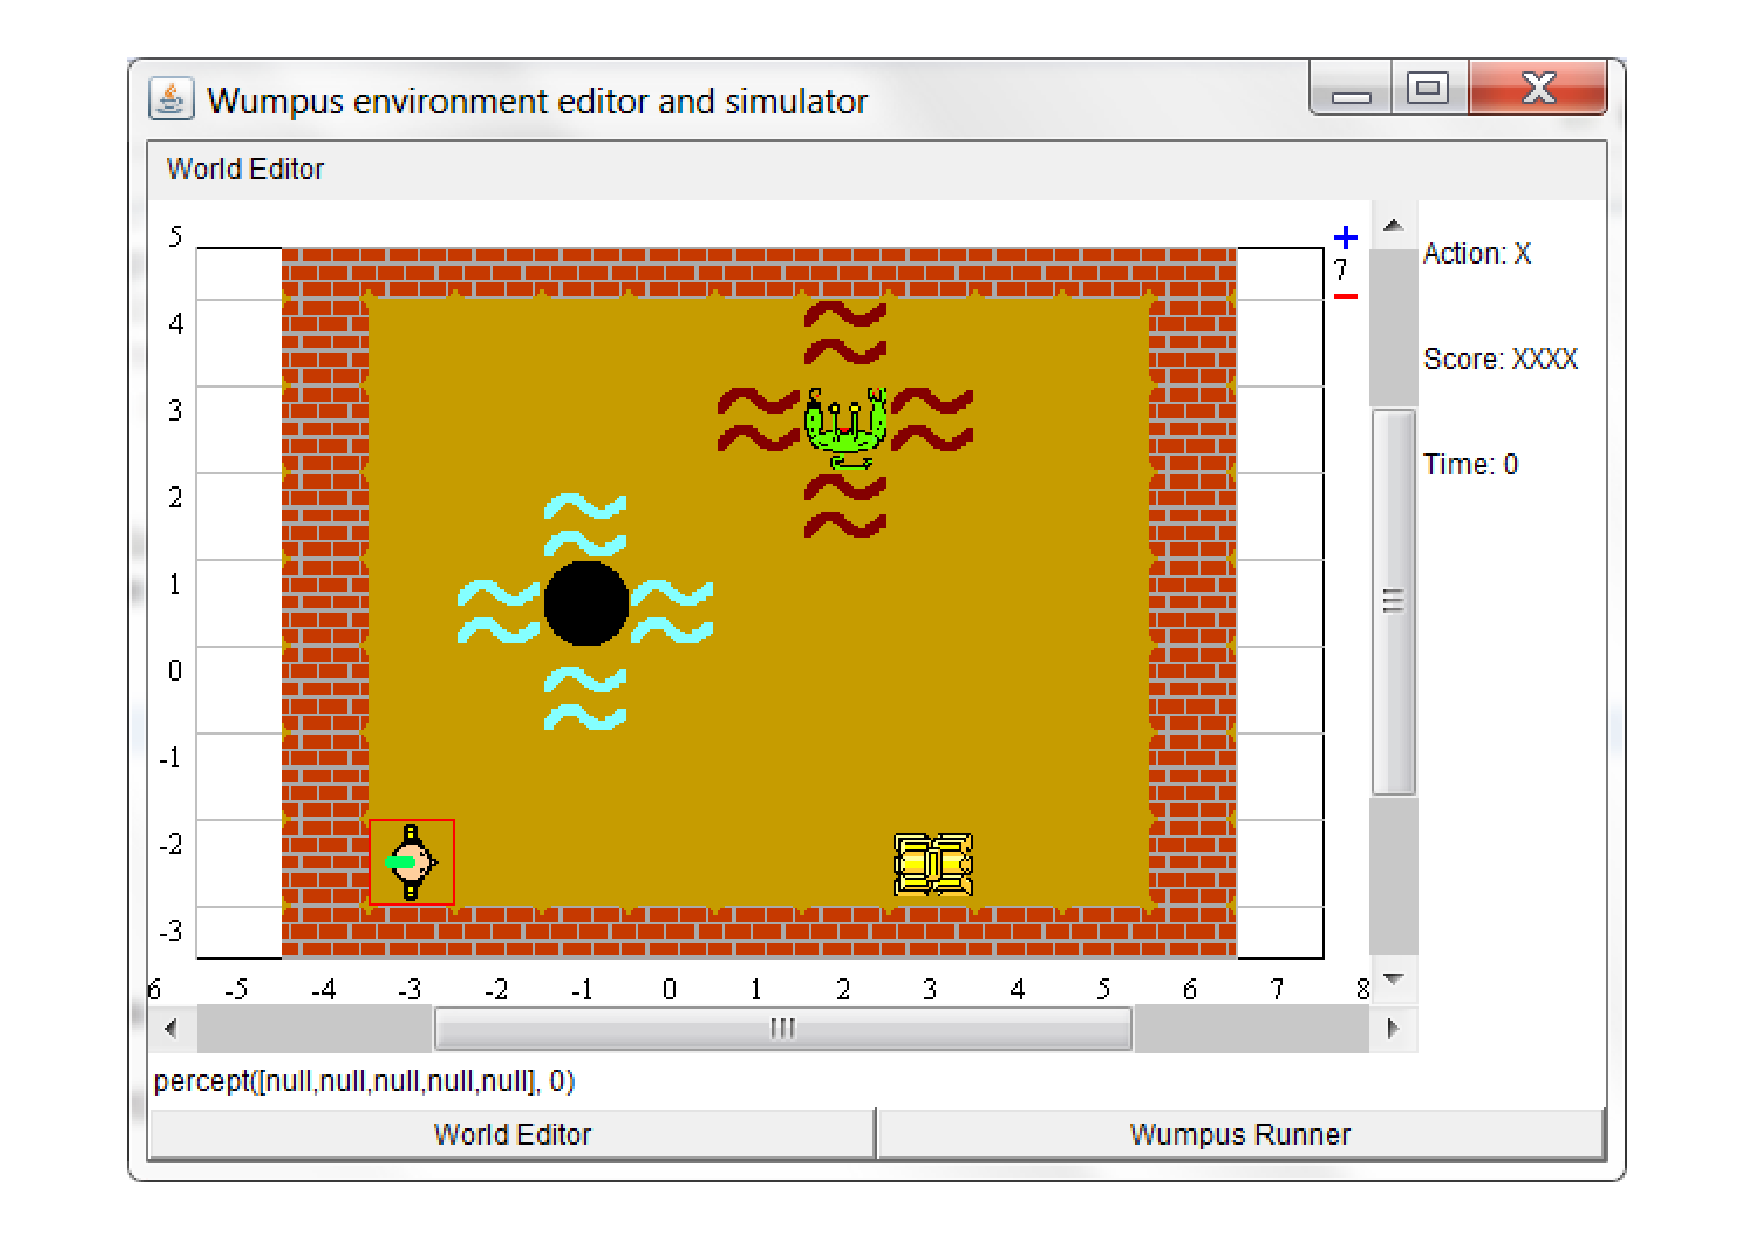
\includegraphics[width=12.5cm]{Figures/wumpusRunner.pdf}
\caption{The Wumpus Runner window}\label{fig:wumpusRunner}
\end{figure}

The Wumpus Runner window differs in that it shows the action last performed, the
score the agent has realized during the game so far, and the current time. Of
course, it is the objective of the game to achieve a score that is as high as
possible.


%
%
%
\section{Perception in the Wumpus World}
%

Your agent is located in a two-dimensional grid-like cave, hoping to
find the pile of gold that is hidden somewhere. As there are pits and
there is the Wumpus, the agent has to be careful however. Falling into a pit or
hitting upon the Wumpus kills the agent immediately and terminates the game. It is known that the
Wumpus is very lazy and never moves which makes exploration a little safer. The Wumpus spreads a nasty smell which
the agent is able to sense just before it hits upon the Wumpus. Moreover, pits
cause some hefty air circulation which the agent can sense as well before it
falls into a pit. Of course, the agent also cannot move through walls and needs to detect walls to be
able to explore the cave. If the agent uses its senses and makes the right inferences,
it is possible to navigate safely through the cave.

When moving around on the grid, the agent receives \textit{percepts} that inform
it about the cave and its dangers. Table \ref{table:percepts} lists all the
percepts that the agent may receive from the Wumpus World environment.

\begin{table}[h]
\centering
\begin{tabular}{ll}
\hline
\textbf{Percept} & \textbf{Explanation}\\
\hline
breeze & Breezes are perceived in each of the four grid cells adjacent to a
pit\\
stench & A stench is perceived in each of the four grid cells adjacent to the
Wumpus\\
bump & A bump is perceived when the agent hits a wall\\
scream & A scream is perceived when the Wumpus dies\\
glitter & A glitter is perceived when the agent is standing on the pile of
gold\\
time(T) & T represents the time or number of rounds in natural numbers 
0,1,2,...\\
\hline
\end{tabular}
\caption{Overview of all Percepts in the Wumpus World}\label{table:percepts}
\end{table}

An agent hits a wall when it performs a forward action and is facing a wall.
Of course, when a scream is perceived it can safely be concluded that the Wumpus
is dead and the Wumpus needs to be no longer feared. The time is incremented
after each action listed below that is performed. Note that the time percept is
the only parameterized percept.

Finally, at the lower left bottom of the Wumpus Runner window the percept sent
is displayed in a slightly different format. Initially, the following is
displayed:
\begin{center}
\verb|percept([null,null,null,null,null],0)|
\end{center}
Here, each of the \verb|null|s indicate that no breeze, stench, bump, scream,
glitter is perceived at time 0, as is to be expected.


%
%
%
\section{Acting in the Wumpus World}
%
The agent can perform a number of actions to achieve its goal of finding the
gold. The agent can only move forward and has to turn left or right to move into
another direction. The agent needs to be explicitly instructed to grab the gold.
Of course, it can only do so when it stands on the cell where the pile of gold
is located and thus first has to locate the pile. Sometimes there is no other
way to reach the pile of gold then by killing the Wumpus. The agent has
exactly one arrow which the agent can shoot at the Wumpus. The agent thus has
exactly one chance to kill the Wumpus. The Wumpus is killed if the arrow hits
it and can move unobstructed in a straight line from the agent towards the
Wumpus. Finally, apart from finding the gold, the agent has the goal to get out
of the cave again (of course preferablly with the gold!). It can do so by the
executing the action climb at the cell the agent started, i.e. the cell the
agent was at time 0. Table \ref{table:actions} lists all actions that are available to the
agent.

\begin{table}[h]
\centering
\begin{tabular}{ll}
\hline
\textbf{Action} & \textbf{Result}\\
\hline
forward & The agent moves one cell in the direction its facing\\
grab & The agent picks up the gold. Only works if he is standing on the pile of
gold\\
shoot & The agent shoots an arrow (only if it still has one)\\
turn(left) & The agent makes a 90 degree left turn\\
turn(right)	& The agent makes a 90 degree right turn\\
climb & The agent climbs out of the cave if positioned at the cell it started
at\\
\hline
\end{tabular}
\caption{Actions in the Wumpus World the Agent can Perform}\label{table:actions}
\end{table}

As discussed, moving is dangerous. If the agent hits upon the Wumpus or falls
into a pit, he will be killed instantly. When the arrow is shot it moves
forward in a straight line up to the first wall or the Wumpus, or it moves on
forever. If the arrow never hits a wall or the Wumpus and continues
forever, the environment may lock up. Finally, if an arrow is shot and
the wumpus is hit, it will be killed instantly. In that case the Wumpus will make a last
scream that will be heard everywhere in the cave. 

Every action will increment the time counter by 1 and will decrease the score
counter by 1. Shooting the arrow costs 10 points. Collecting the gold
gives 1000 points. The game is over if the agent has climbed out of the cave.
Note that getting back to this position also costs points. The agent may
climb out of the cave any time it wants to. If he does so without having
found the gold, we say the agent ``wuzzes''.

%
%
%
\section{Environment Interface Standard}
%
Upon launching the Wumpus World from \GOAL by starting a multi-agent system, an
initialization can be performed. For the Wumpus World, an initial world can be
loaded by including the following command in the environment section of a
\verb|.mas| file immediately after the reference to the environment file:
\begin{center}
\verb|init [file = "worlds/wumpus.kt1.wld"].|
\end{center}
The reference to the \verb|.wld| file is relative to the directory where the wumpusenvironment jar file is located.
You can use an absolute file reference but this is not recommended. 

The Wumpus World has been \textit{eisified}, meaning that it is an environment
that supports the Environment Interface Standard (EIS; \cite{Beh10,EISurl}).
This means that you can use in combination with any system such as \GOAL that
supports EIS.


\bibliographystyle{plain}
\bibliography{references}

\end{document}